\documentclass[10pt]{beamer}

\usetheme{metropolis}
\usepackage{appendixnumberbeamer}

\usepackage{booktabs}
\usepackage[scale=2]{ccicons}

\usepackage{pgfplots}
\usepgfplotslibrary{dateplot}

\usepackage{pgfpages}
%\setbeameroption{show notes} %Notizen anzeigen
%\setbeameroption{show notes on second screen = left}


\usepackage{xspace}
\newcommand{\themename}{\textbf{\textsc{metropolis}}\xspace}

\usepackage{color}

\definecolor{codegreen}{rgb}{0,0.6,0}
\definecolor{codegray}{rgb}{0.5,0.5,0.5}
\definecolor{codepurple}{rgb}{0.58,0,0.82}
\definecolor{backcolour}{rgb}{0.95,0.95,0.92}
\definecolor{airforceblue}{rgb}{0.36, 0.54, 0.66}
\definecolor{maroon}{rgb}{0.5, 0.0, 0.0}

\usepackage{listings}
\lstdefinestyle{mystyle}{
	backgroundcolor=\color{backcolour},   
	commentstyle=\color{codegreen},
	keywordstyle=\color{magenta},
	numberstyle=\tiny\color{codegray},
	stringstyle=\color{codepurple},
	basicstyle=\fontsize{8}{10}\selectfont\ttfamily,
	breakatwhitespace=false,         
	breaklines=true,                 
	captionpos=b,                    
	keepspaces=true,                 
	numbers=left,                    
	numbersep=5pt,                  
	showspaces=false,                
	showstringspaces=false,
	showtabs=false,                  
	tabsize=2
}
\lstset{style=mystyle}

\usepackage{diagbox}


\title{Rucksack Problem}
\subtitle{Algorithmen und Datenstrukturen II}
\date{\today}
\author{Sebastian Baumann, Korbinian Karl, Ehsan Moslehi}
\institute{Hochschule für Angewandte Wissenschaften München}
%\titlegraphic{\hfill\includegraphics[height=1.5cm]{logo.pdf}}

\begin{document}

\maketitle

\begin{frame}{Table of contents}
  \setbeamertemplate{section in toc}[sections numbered]
  \tableofcontents[hideallsubsections]
\end{frame}

\section{Beschreibung des Problems}

\begin{frame}[fragile]{Rucksack Problem}
	\begin{figure}
		\centering
		
\includegraphics[width=1\linewidth]{images/rp}
		\caption{Rucksack Problem}
		\label{fig:rp}
	\end{figure}
\end{frame}

\begin{frame}[fragile]{Mathematische Beschreibung}
	\textbf{Gegeben:}
	\begin{itemize}
		\item Ggegenstände $1, 2, 3 , ..., n$
			\begin{itemize}
				\item $w_{i}$ : Wert vom Gegenstand $i$
				\item $v_{i} \in \mathbb{N}$ : Volumen vom Gegenstand $i$
			\end{itemize}
		\item Rucksack mit dem Volumen $V \in \mathbb{N}$
	\end{itemize}
	
	\textbf{Gesucht:}\\ 
	\vspace{0.3cm}
	\hspace{0.3cm}
	Eine Rucksackfüllung mit maximalen Gesamtwert, wobei das Volumen $V$ nicht überschritten werden darf.\\
	\vspace{0.3cm}
	\begin{center}
		$max \Big\lbrace \sum \limits_{i=1}^{n} w_{i}t_{i} \mid \sum \limits_{i=1}^{n} v_{i}t_{i} \leq V , \forall i : t_{i} \in \{0, 1\} \Big\rbrace$
	\end{center}
\end{frame}

\begin{frame}[fragile]{Mathematische Beschreibung}
	\begin{itemize}[<+- | alert@+>]
		\item[] \begin{center}
			Ganzzahliges Lineares Optimierungsproblem
		\end{center}
		\item[] \begin{center}
			\textbf{NP-Vollständig}
		\end{center}
	\end{itemize}
\end{frame}

\section{Lösungsansätze}

\begin{frame}[fragile]{Brute Force}
	\begin{enumerate}
		\item Brute Force
		\item Greedy
		\item Dynamische Programmierung 
	\end{enumerate}
\end{frame}

\section*{Brute Force}

\begin{frame}[fragile]{Brute Force}
	\begin{figure}
		\centering
		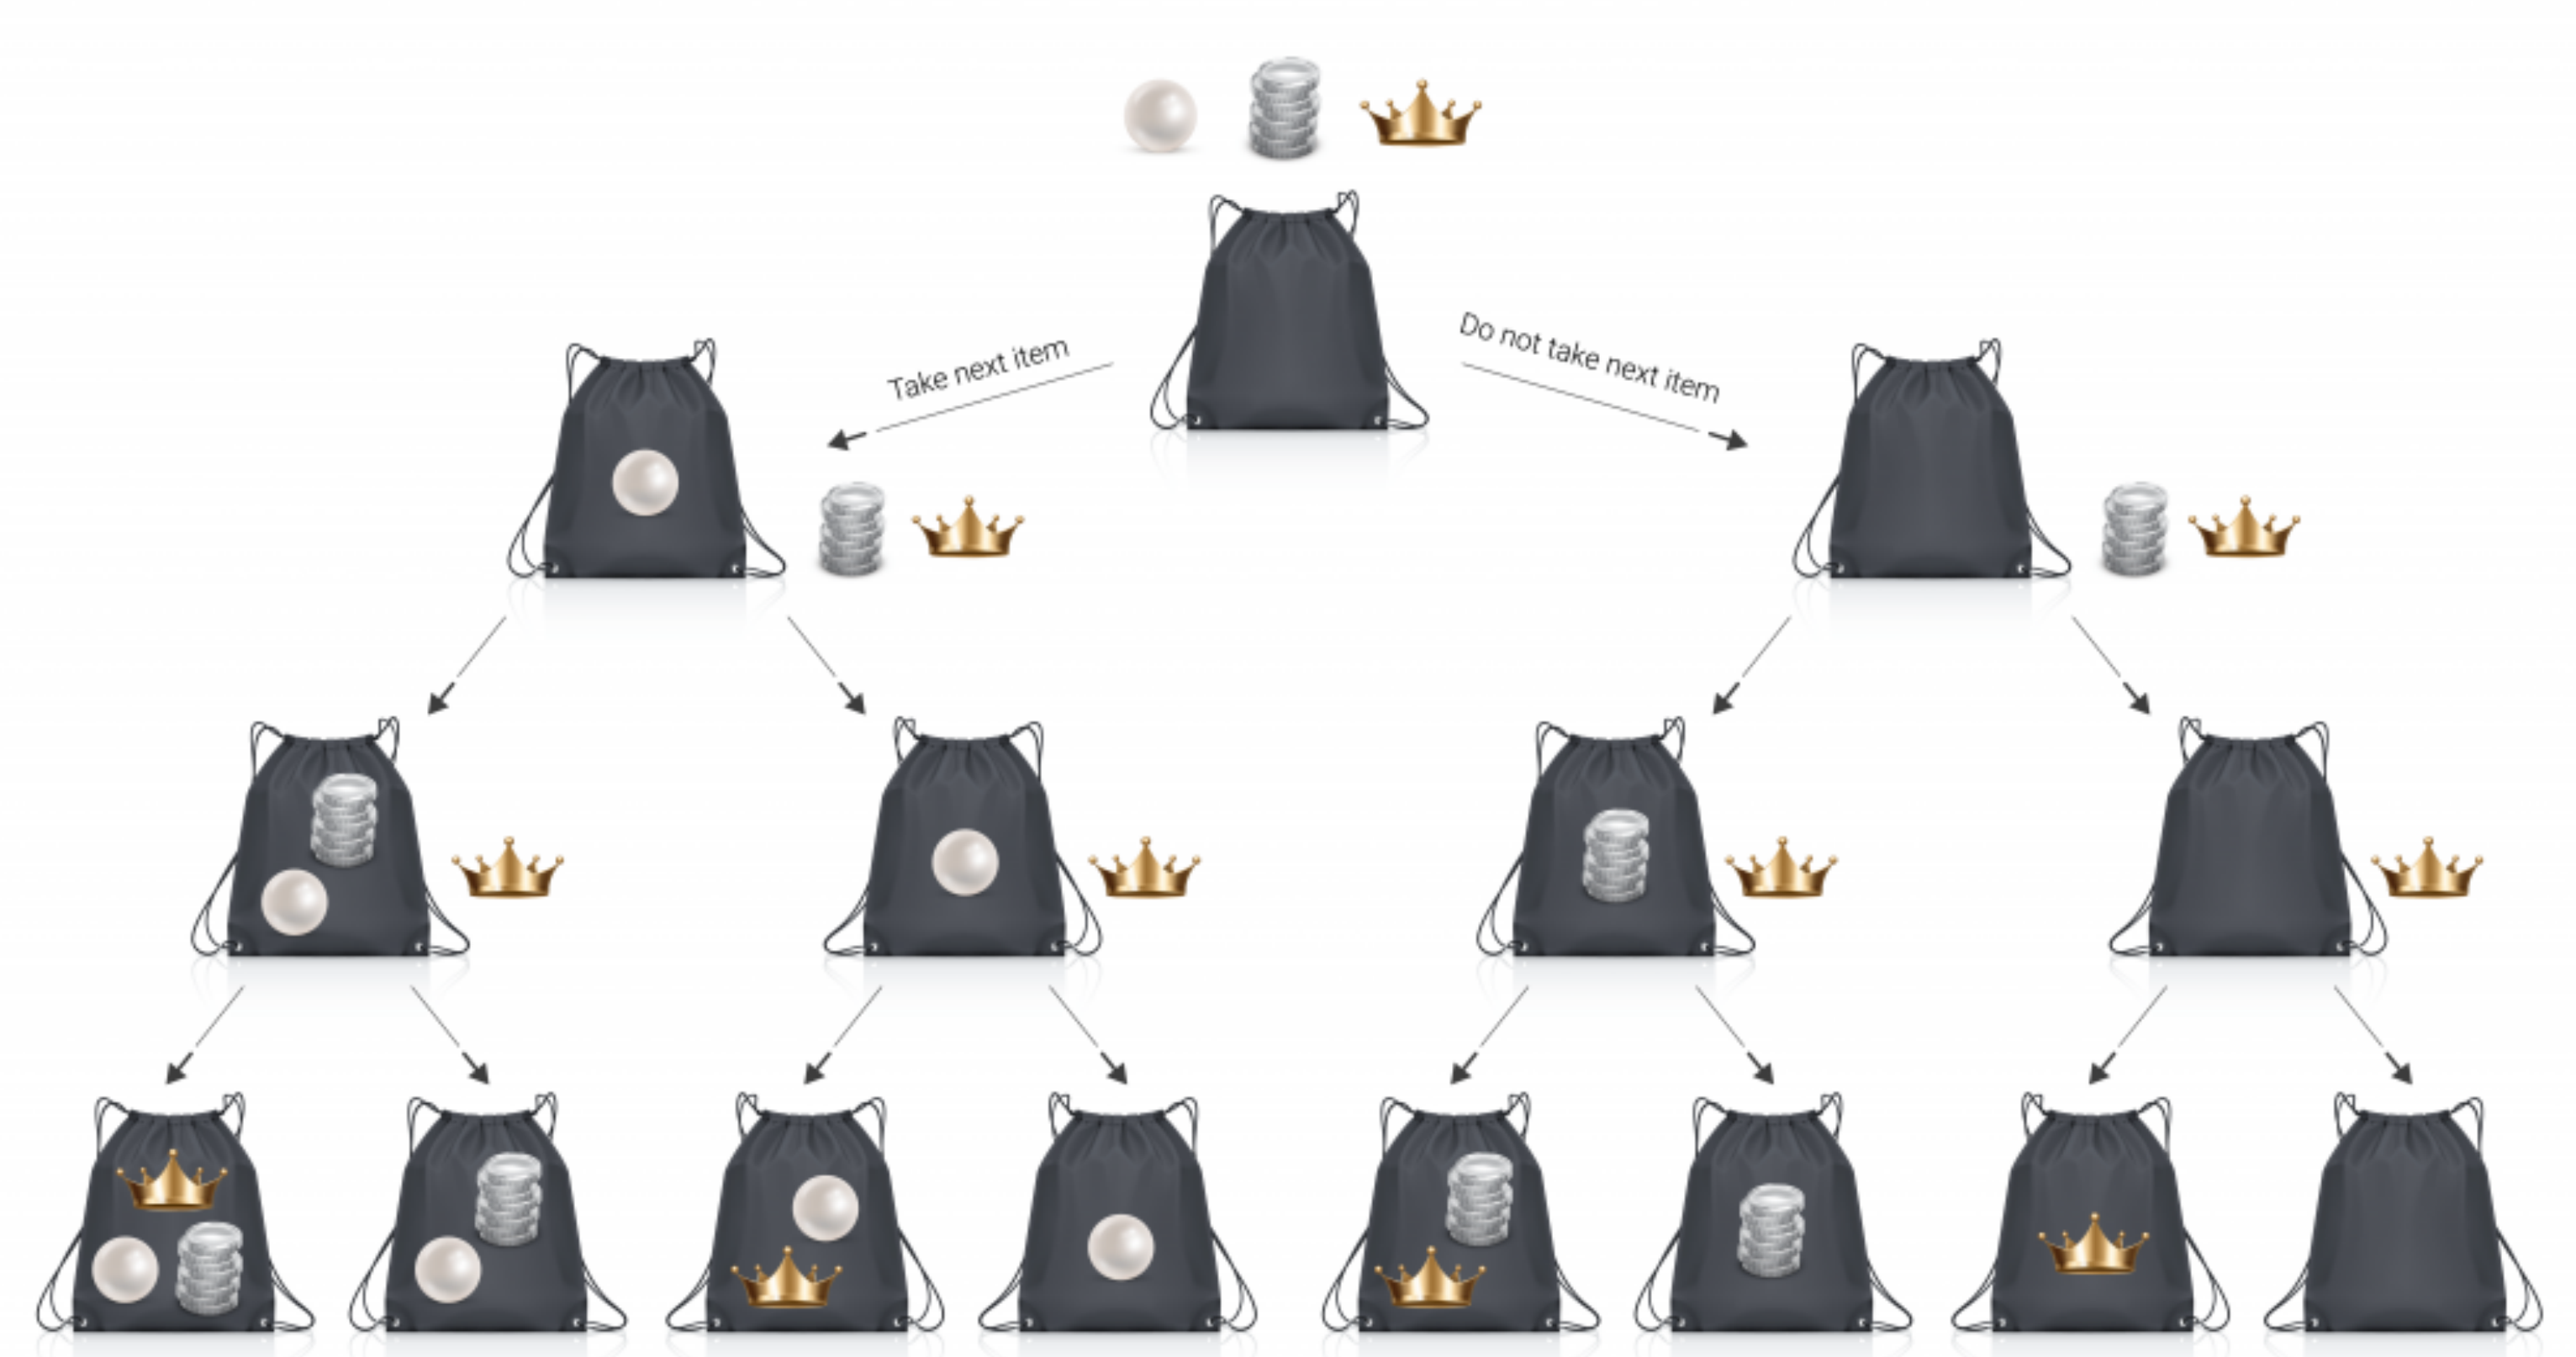
\includegraphics[width=1\linewidth]{images/rp-bf}
		\caption{Probiere alle Teilmengen!}
		\label{fig:rp-bf}
	\end{figure}
\end{frame}

\begin{frame}[fragile]{Brute Force}
	\begin{itemize}[<+- | alert@+>]
		\item[] \begin{center}
			\textbf{Optimale globale Lösung wird gefunden.}
		\end{center}
	\vspace{1cm}
		\item[] \begin{center}
			\textbf{Exponentielle Laufzeit $O(2^n)$}
		\end{center}
	\end{itemize}
\end{frame}

\section*{Greedy Algorithmus}

\begin{frame}[fragile]{Greedy Strategie}
	\textbf{Strategien:}
	\begin{enumerate}[<+- | alert@+>]
		\item \textbf{Absteigende Sortierung nach Wert}
		\item \textbf{Aufsteigende Sortierung nach Volumen}
		\item \textbf{Absteigende Sortierung nach Wertdichte} \Large{ $d_{i} = \frac{w_{i}}{v_{i}}$}
	\end{enumerate}
	\vspace{1cm}
	\textbf{Packe solange Gegenstände in den Rucksack, bis kein Gegenstand mehr rein passt!}
\end{frame}

\begin{frame}[fragile]{Greedy Strategie}
	\begin{itemize}[<+- | alert@+>]
		\item[] \begin{center}
			\textbf{Optimale globale Lösung wird \Large{NICHT} \normalsize{gefunden}.}\\
			\textbf{Optimale lokale Lösung wird gefunden.}
		\end{center}
		\vspace{1cm}
		\item[] \begin{center}
			\textbf{Laufzeit $O(n. \log n)$}
		\end{center}
	\end{itemize}
\end{frame}

\section*{Dynamische Programmierung}

\begin{frame}[fragile]{Dynamische Programmierung}
	\begin{tabular}{|l||c|c|c|c|}
		\hline
		\diagbox{I:}{V:}
		& 0 & 1 & 2 & 3 \\
		\hline
		\hline
		0	&    0    &     0     &      0      &       0     \\
		\hline
		1	&    0    &     0     &      0      &       0     \\
		\hline
		2	&    0    &     0     &      0      &       0     \\
		\hline
		3	&    0    &     0     &      0      &       0     \\
		\hline
		4	&    0    &     0     &      0      &       0     \\
		\hline
		5	&    0    &     0     &      0      &       0     \\
		\hline
	\end{tabular}


\end{frame}

\begin{frame}[standout]
  Fragen?
\end{frame}

\appendix

%\begin{frame}[allowframebreaks]{References}
%  \bibliography{demo}
%  \bibliographystyle{abbrv}
%\end{frame}

\end{document}
